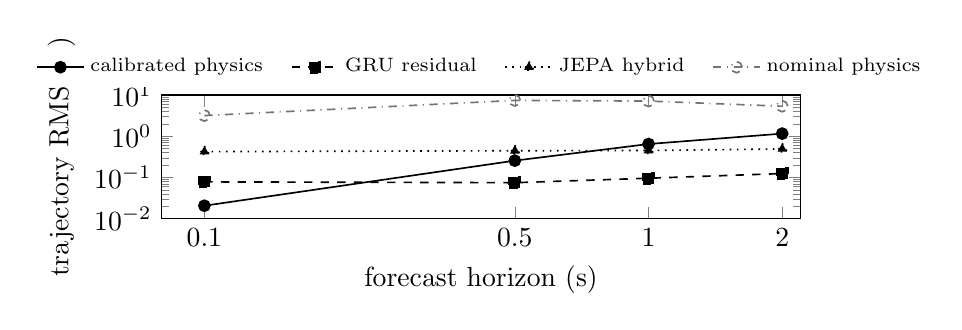
\begin{tikzpicture}
\begin{axis}[width=0.80\textwidth,height=0.26\textwidth, xmode=log, ymode=log, xlabel={forecast horizon (s)}, ylabel={trajectory RMSE (\si{\radian\per\second})}, xmin=.08,xmax=2.2,ymin=.01,ymax=10, xtick={.1,.5,1,2}, xticklabels={$0.1$,$0.5$,$1$,$2$}, grid=none, minor tick num=1, legend style={font=\scriptsize, draw=none, at={(0.5,1.06)}, anchor=south, legend columns=4,/tikz/every even column/.append style={column sep=0.8em}}]
  \addplot[black, solid, semithick, mark=*] coordinates {(.1,.0207) (.5,.2566) (1,.6487) (2,1.1603)}; \addlegendentry{calibrated physics}
  \addplot[black, dashed, semithick, mark=square*] coordinates {(.1,.0784) (.5,.0749) (1,.0961) (2,.1248)}; \addlegendentry{GRU residual}
  \addplot[black, dotted, semithick, mark=triangle*] coordinates {(.1,.4244) (.5,.4455) (1,.4523) (2,.4933)}; \addlegendentry{JEPA hybrid}
  \addplot[black!55, dashdotted, semithick, mark=o] coordinates {(.1,3.177) (.5,7.409) (1,7.142) (2,5.362)}; \addlegendentry{nominal physics}
\end{axis}
\end{tikzpicture}
